\section{Experiments}
% (recommended size: 1.5 pages)
	In this section, we will first describe the realistic simulation of clients connecting/disconnecting from the server, a requirement of the customer WantGame BV. After that, we first discuss our experimental setup. Finally, we describe the experiments we have conducted on FDDG and the outcome of these experiments.
	
\subsection{Simulation of connecting/disconnecting clients}
\label{subsec:simulation_clients}
A requirement of our game is that a realistic game trace should be used to simulate the behavior of clients connecting and disconnecting to and from the server.
A potential data set with game traces we can use is described in the paper of Guo et al. \cite{guo2012game}.
Here, the design of the GTA (Game Trace Archive) is explained and possible applications of the data are discussed.
Amongst the genres of the analyzed games are Massively Multiplayer Online Role-Playing Game (MMORPGs), board games and Real-time Strategy (RTS) games. 
Since our games closely resembles a MMORPG, we decided to use the WoWAH game trace \cite{lee2011world}.
This game trace archive contains data about 91065 players during 1107 days. The dataset is available as a free download on their website\footnote{http://mmnet.iis.sinica.edu.tw/dl/wowah/}.
We gathered data about the number of online players during 24 hours. 
A visual representation of the amount of online avatars in the game trace can be found in Figure \ref{fig:online_players_plot}. As we see, the number of online players is minimal during the morning and maximal around midnight.

\begin{figure}[h!]
  \centering
    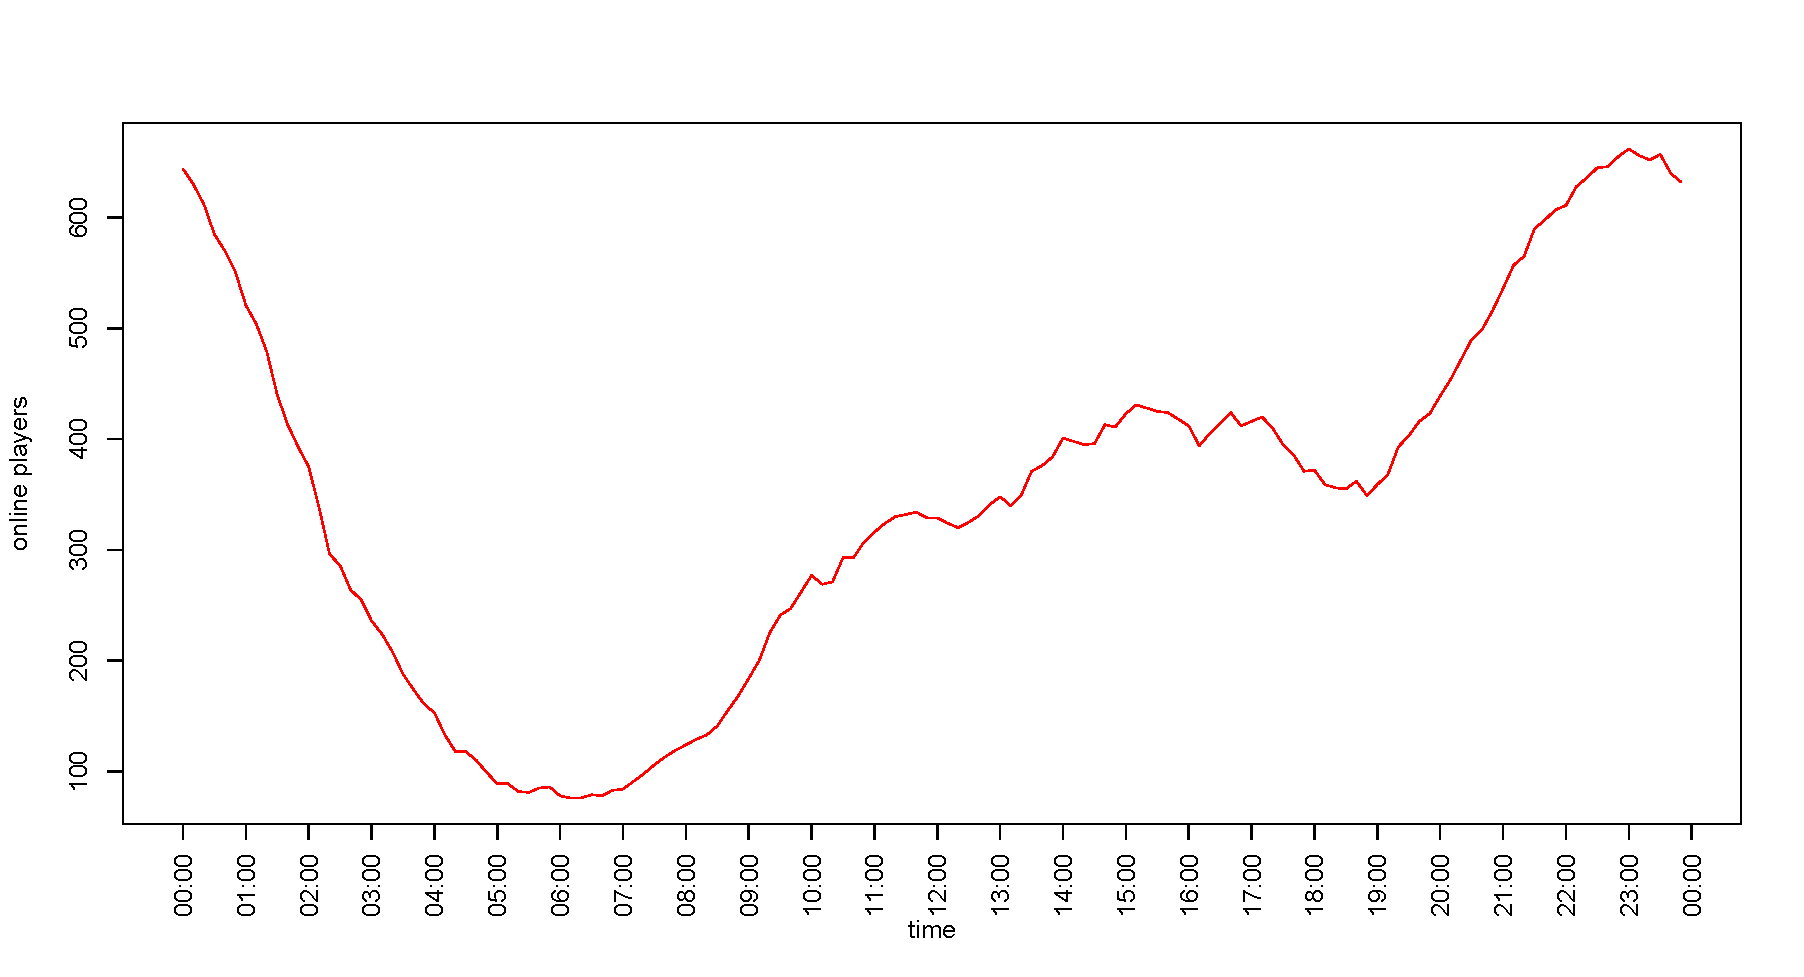
\includegraphics[width=\textwidth]{images/online_players_plot}
    
  \caption{The number of online players during 24 hours (2007-07-14)}
  \label{fig:online_players_plot}
\end{figure}

We keep track of the number of players connecting and disconnecting during 10-minute time intervals.
We used that interval because in the WoWAH dataset, samples are taken every 10 minutes.
Using this data, we were able to create a realistic pattern of players connecting and disconnecting to and from the game.
A simulation file has been created, containing information about all events during 24 hours. This file can be used to actually run the simulation of connecting and disconnecting players.

\subsection{Experimental setup}
\label{subsec:experimental_setup}
% Describe the working environments (DAS-4, Amazon EC2,
% etc.), the general workload and monitoring tools and libraries, other tools and
% libraries you have used to implement and deploy your system, other tools and
% libraries used to conduct your experiments.

	Since FDDG is a lightweight game, we can easily simulate it on our desktop computers with 5 servers, 100 clients and 20 dragons. 
	We decided to simulate the game on an iMac (late 2013 edition), with 8 Intel core i7 3.5 GHz processors and 16 GB (1600 MHz DDR3) RAM memory. 
	This gave us easier access and allowed better monitoring of performance.
	We haven't used the DAS cluster nor Amazon's EC2 platform service to run experiments on. 
	Note that we did test a truly distributed system by using three??? laptops and one desktop computer.
	
	FDDG makes use of Java's Remote Method Invocation (RMI) to call methods on objects running on remote machines with locally specified parameters. 
	Furthermore, we've developed our own message system that makes use of \emph{actions} to implement updates and acknowledgments.
	
	A simulation starts as soon as the first client joins the server. The game is then considered active and will run until either all players are dead or all dragons are slain.


\subsection{Experiments}
\label{subsec:experiments}
% Describe the experiments you have conducted to analyze each
% system feature, such as consistency, scalability, fault-tolerance, and
% performance. Analyze the results obtained for each system feature. Use one
% sub-section per experiment (or feature). In the analysis, also report:
% i. Service metrics of the experiment, such as runtime and response time of
% the service, etc.
% ii. (optional) Usage metrics and costs of the experiment.
	We ran experiments concerning the consistency, fault-tolerance and scalability of the game. Below are the results of the experiments conducted for each of these features.

	\subsubsection{Consistency}
	\label{subsubsec:consistency}
		In order to test consistency, we ran the simulation with exactly the same setup multiple times.
		We checked if the result was consistent, that is the same field state at the end of each simulation. 
		
	\subsubsection{Fault-tolerant}
	\label{subsubsec:fault-tolerant}
		To test fault-tolerance, we ran the following scenarios:
		\begin{enumerate}
			\item During simulation we killed some client nodes. The servers should then remove the players from the field and continue the game.
			\item During the simulation we killed one server and let it recover. It then should connect to the other servers, receive the current field and start participating again.
			\item We simulated the loss of move actions with a small percentage server side. We then checked if in the next update, the field became consistent again when the next movement was received.
		\end{enumerate}
		
		The results are as follows... 
		
	\subsubsection{Scalability}
	\label{subsubsec:scalability}
		The minimum requirements of 5 servers, 100 clients and 20 dragons were easily fulfilled. We therefore decided to try 10 dragons, 200 clients and 40 dragons (twice as much for every parameter). The results were ...
